% ============================================================================
%  CAPÍTULO III: DESARROLLO DEL TRABAJO
% ============================================================================

\section{Desarrollo del Trabajo}

\subsection{Propuesta y Análisis Técnico de Herramientas Open Source}

En el ámbito de la seguridad perimetral y el monitoreo defensivo de redes, existen múltiples herramientas de código abierto destinadas a la inspección de tráfico. Para satisfacer los requerimientos de la presente actividad, se seleccionaron para una comparativa técnica profunda dos plataformas de renombre internacional: \textbf{Suricata} y \textbf{Snort 3}, complementadas con una revisión metodológica de \textbf{Wireshark} como analizador forense interactivo.

\subsubsection{Análisis Técnico de Suricata 7}

Desarrollado y mantenido por la \textit{Open Information Security Foundation} (OISF), Suricata es un motor de seguridad de red de código abierto de nueva generación que integra de forma unificada capacidades de IDS, IPS y Monitoreo de Seguridad de Red (\textit{Network Security Monitoring}, NSM) \citep{oisf_suricata_2024}. Sus características técnicas distintivas incluyen:

\begin{itemize}
  \item \textbf{Arquitectura Multihilo Nativa (*True Multi-Threading*):} A diferencia de motores monocatenarios históricos, Suricata fue diseñado desde su origen para distribuir de forma eficiente y paralela la carga de procesamiento entre todos los núcleos de CPU disponibles en el sistema operativo. Emplea un esquema de afinidad de CPU (\textit{CPU Pinning}) que permite asignar hilos específicos para la adquisición de paquetes, la decodificación de protocolos, la aplicación de firmas y el volcado de registros en disco, mitigando drásticamente el riesgo de pérdida de paquetes (\textit{packet drops}) en enlaces de alta velocidad.
  \item \textbf{Aceleración de Patrones con Intel Hyperscan:} Integra de forma nativa la biblioteca de expresiones regulares de alto rendimiento \textbf{Hyperscan} \citep{intel_hyperscan_2019}. Esta tecnología aprovecha instrucciones vectoriales del procesador (como AVX2 y AVX-512) para evaluar decenas de miles de firmas concurrentemente en un único paso de inspección, alcanzando tasas de escaneo de múltiples gigabits por segundo sin degradación de latencia.
  \item \textbf{Modos de Adquisición Dual (IDS e IPS):} En modo pasivo (IDS), interactúa directamente con los anillos de memoria del kernel mediante zócalos de alto desempeño \texttt{AF\_PACKET} con búferes en anillo (\textit{ring buffers}). En modo prevención (IPS), se enlaza de forma transparente con el subsistema \textbf{NFQUEUE} del cortafuegos \texttt{nftables} de Linux, permitiendo que las firmas con acción \texttt{drop} descarten físicamente los paquetes anómalos antes de que ingresen a la pila TCP/IP local.
  \item \textbf{Decodificación Profunda de Protocolos de Directorio Activo:} Posee decodificadores internos altamente especializados para protocolos corporativos fundamentales: \textbf{Kerberos (puerto 88)}, \textbf{LDAP (puertos 389 y 636)}, \textbf{DCERPC} y \textbf{SMB/CIFS (puerto 445)}. Esta capacidad resulta crucial para detectar ataques dirigidos contra controladores de dominio Windows o Samba 4, tales como transferencias de archivos sospechosas hacia carpetas compartidas (\textit{shares}), sondeos anómalos o intentos de enumeración de cuentas.
  \item \textbf{Telemetría Estructurada EVE JSON:} Genera salidas en formato \textbf{EVE} (\textit{Extensible Event Format}), un estándar en formato JSON unificado que registra metadatos de sesiones HTTP, transacciones DNS, certificados TLS, anomalías de flujo y eventos de descarte (\texttt{drop}), lo que facilita su indexación directa en consolas SIEM, Elasticsearch, Zabbix o Grafana.
\end{itemize}

\subsubsection{Análisis Técnico de Snort 3}

Desarrollado bajo el liderazgo de Cisco Talos, Snort ha sido históricamente el estándar de facto en detección de intrusiones en redes IP \citep{caswell_snort_2007}. En su versión más reciente, \textbf{Snort 3}, la plataforma experimentó una reescritura arquitectónica total para resolver las limitaciones de escalabilidad de Snort 2 \citep{cisco_snort3_2024}:

\begin{itemize}
  \item \textbf{Evolución hacia Modelo Multihilo:} Snort 3 abandona el modelo monohilo tradicional que obligaba a ejecutar múltiples instancias independientes del proceso coordinadas externamente. Introduce una arquitectura multihilo modular basada en hilos de procesamiento de paquetes coordinados que comparten una tabla global de configuración e información de estado.
  \item \textbf{Configuración Basada en Lenguaje Lua:} Reemplaza la sintaxis rígida del archivo \texttt{snort.conf} por scripts en lenguaje \textbf{Lua} (\texttt{snort.lua}). Esto dota al motor de una modularidad sin precedentes, permitiendo declarar tablas dinámicas, inspectores de protocolos personalizados y estructuras condicionales en el arranque del servicio.
  \item \textbf{Capa de Adquisición de Datos DAQ (*Data Acquisition*):} Snort 3 desacopla la lógica de captura mediante el subsistema DAQ, el cual ofrece controladores modulares para interfaces de red (\texttt{daq\_pcap}, \texttt{daq\_afpacket}, \texttt{daq\_nfq}). Para operar como IPS en sistemas Linux, depende del módulo \texttt{daq\_nfq} para interactuar con las colas de Netfilter.
  \item \textbf{Inspectores de Protocolo Mejorados:} Incorpora inspectores avanzados de nueva generación para el manejo de sesiones TCP, reensamblaje de flujos IP y normalización de transacciones HTTP.
\end{itemize}

\subsubsection{Rol Complementario de Wireshark}

Si bien el alcance de un IDS/IPS radica en la inspección desatendida y autónoma de flujos masivos de red mediante reglas automatizadas, herramientas como \textbf{Wireshark} \citep{combs_wireshark_2020} desempeñan un rol defensivo complementario indispensable:

\begin{itemize}
  \item \textbf{Análisis Forense Profundo Interactivo:} Wireshark no actúa como un motor de descarte o alerta continua en un servidor de producción, sino como una herramienta de análisis forense en diferido. Permite a los analistas de seguridad abrir capturas completas de paquetes (\textit{PCAP}) generadas por un sensor IDS para diseccionar campos de encabezado bit a bit, evaluar secuencias TCP anómalas y reconstruir cargas útiles comprometidas.
  \item \textbf{Validación de Firmas:} Resulta esencial durante la fase de desarrollo y prueba de reglas de detección, permitiendo verificar que los campos de coincidencia (\texttt{content}, \texttt{byte\_test}, \texttt{pcre}) coincidan exactamente con la estructura de red del exploit evaluado.
\end{itemize}

\subsubsection{Comparativa Técnica Profunda: Suricata vs Snort 3}

A fin de brindar un análisis riguroso y objetivo, la Tabla~\ref{tab:comparativa-suricata-snort} resume la evaluación comparativa de ambas herramientas a lo largo de diez dimensiones técnicas críticas.

\begin{table}[H]
\centering
\caption{Comparativa Técnica Detallada entre Suricata 7 y Snort 3}
\label{tab:comparativa-suricata-snort}
\contenidoConFuente{%
  \begin{tablaAPA}
  \begin{tabular}{L{2.8cm}L{5.8cm}L{5.8cm}}
  \toprule
  \textbf{Criterio Técnico} & \textbf{Suricata (Versión 7.x)} & \textbf{Snort 3 (Versión 3.x)} \\
  \midrule
  \textbf{Arquitectura de Hilos} & Multihilo nativo y simétrico con afinidad de núcleos (\textit{flow pinning}). Distribuye automáticamente los flujos en toda la CPU. & Multihilo modular basado en hilos de procesamiento que comparten estado común a través de la capa DAQ. \\
  \textbf{Aceleración de Patrones} & Integración nativa optimizada de \textbf{Intel Hyperscan} (AVX2/AVX-512) y Aho-Corasick. & Soporte de Hyperscan y algoritmos AC-BNFA mediante configuración modular en Lua. \\
  \textbf{Mecanismo IPS en Linux} & Integración directa y nativa con \textbf{NFQUEUE} (\texttt{libnetfilter\_queue}) y cortafuegos \texttt{nftables}. & Requiere la capa intermedia DAQ mediante el módulo \texttt{daq\_nfq}. \\
  \textbf{Inspección de Protocolos AD} & Decodificación profunda nativa de \textbf{SMB (445), Kerberos (88), LDAP (389) y DCERPC}. & Cobertura enfocada en HTTP/TCP/UDP. La inspección SMB avanzada es más reciente y dependiente de preprocesadores. \\
  \textbf{Telemetría y Registro} & Formato unificado \textbf{EVE JSON} nativo (\texttt{eve.json}) con detalles de alertas, flujos, TLS, DNS y eventos \texttt{drop}. & Soporte nativo de salida JSON (\texttt{alert\_json}), además del formato binario Unified2 y texto plano. \\
  \textbf{Disponibilidad en Debian} & \textbf{Paquete oficial de primera clase} en Debian 12 y 13 (\texttt{apt install suricata suricata-update}). & No disponible en repositorios oficiales base de Debian 12/13; requiere compilación manual o contenedores Docker. \\
  \textbf{Lenguaje de Configuración} & Sintaxis estandarizada y legible en \textbf{YAML} (\texttt{suricata.yaml}). & Lenguaje de programación interpretado \textbf{Lua} (\texttt{snort.lua}), altamente flexible pero más complejo. \\
  \textbf{Ecosistema de Firmas} & Total compatibilidad con conjuntos de reglas de \textbf{Emerging Threats (ET Open/Pro)} y gestión con \texttt{suricata-update}. & Conjuntos de reglas de \textbf{Cisco Talos VRT} y compatibilidad con reglas de la comunidad. \\
  \textbf{Monitoreo de Archivos} & Capacidad nativa de extracción y cálculo de hashes MD5/SHA256 de archivos en tránsito en protocolos SMB/HTTP. & Requiere inspectores específicos de archivos configurados dentro de la cadena Lua. \\
  \textbf{Resiliencia ante Fallos} & Soporte directo del flag \texttt{bypass} en \texttt{nftables} que garantiza continuidad operativa (\textit{Fail-Open}). & Soporte de tolerancia a fallos dependiente del modo de operación del módulo DAQ seleccionado. \\
  \bottomrule
  \end{tabular}
  \end{tablaAPA}%
}{Elaboración propia con base en \cite{oisf_suricata_2024} y \cite{cisco_snort3_2024}.}
\end{table}

\subsubsection{Justificación de Selección para la Infraestructura Corporativa}

Con base en la evaluación técnica previa, se determinó seleccionar \textbf{Suricata 7} como la plataforma defensiva nativa de producción para la infraestructura centralizada en el servidor corporativo \texttt{dc1} (\texttt{192.168.0.2}), manteniendo a \textbf{Snort 3} como entorno comparativo en contenedor y a \textbf{Wireshark} como plataforma forense de auditoría. Las razones determinantes que sustentan esta decisión de ingeniería son:

\begin{enumerate}
  \item \textbf{Especialización en Protocolos de Identidad y Active Directory:} El servidor \texttt{dc1} aloja el Controlador de Dominio de la organización (\texttt{SUDOERS.LAN}) sobre Samba 4 nativo. Suricata integra decodificadores de protocolo de capa 7 altamente maduros y nativos para \textbf{SMB/CIFS (puerto 445)}, \textbf{Kerberos (puerto 88)}, \textbf{LDAP (puertos 389/636)} y \textbf{DCERPC}. Esta capacidad le permite inspeccionar transacciones de autenticación, aperturas de recursos compartidos y consultas de directorio sin requerir software propietario adicional ni preprocesadores externos complejos, detectando tempranamente técnicas de abuso de identidad como \textit{Kerberoasting}, ataques de paso de ticket (*Pass-the-Ticket*) o explotación de fallos en SMB.
  \item \textbf{Soporte Oficial, Estabilidad y Mantenibilidad en Debian:} Suricata es un paquete de primera clase plenamente empaquetado y mantenido en los repositorios oficiales de Debian GNU/Linux 12 (Bookworm) y 13 (Trixie). Su despliegue nativo permite una integración limpia con el gestor del sistema \texttt{systemd}, aislamiento de privilegios de usuario y un ciclo de actualización de firmas completamente automatizado mediante \texttt{suricata-update}. Por el contrario, desplegar Snort 3 en Debian demanda la compilación manual de múltiples dependencias o el uso de contenedores Docker con privilegios elevados de red (\texttt{network\_mode: host} y capacidades \texttt{CAP\_NET\_ADMIN}), lo que incrementa la superficie de ataque y la complejidad operativa.
  \item \textbf{Concurrencia Simétrica y Desempeño Multihilo:} La arquitectura de hilos de Suricata distribuye automáticamente los flujos de red entrantes entre todos los núcleos de CPU del servidor físico mediante afinidad de procesamiento (\textit{CPU flow pinning}). Al combinar esta característica con el motor de búsqueda vectorial \textbf{Intel Hyperscan}, Suricata procesa decenas de miles de reglas concurrentemente sin degradar el rendimiento ni introducir cuellos de botella en transferencias masivas de archivos por SMB ni en el tráfico web HTTPS.
  \item \textbf{Integración Directa y Transparente con Netfilter/NFQUEUE:} Suricata interactúa de manera directa con las colas de paquetes en espacio de kernel (\texttt{NFQUEUE}) provistas por \texttt{nftables}, permitiendo alternar de forma dinámica entre un modo IDS puramente observador y un modo IPS de prevención activa. La inclusión de la directiva \texttt{bypass} en la regla del cortafuegos garantiza resiliencia operativa (*Fail-Open*): si el proceso de Suricata se detiene o reinicia, el kernel permite el paso inmediato del tráfico legítimo, previniendo denegaciones de servicio autoinfligidas.
  \item \textbf{Telemetría Estructurada en EVE JSON:} La salida estándar en formato JSON (\texttt{eve.json}) genera registros detallados con metadatos de flujo, identidades de usuario, huellas TLS y veredictos de descarte (\texttt{drop}), lo que posibilita una integración directa con el servidor de monitoreo Zabbix (\texttt{192.168.0.3}) y futuras plataformas SIEM corporativas.
\end{enumerate}

% ----------------------------------------------------------------------------
\subsection{Propuesta Arquitectónica: Ubicación del Monitor en la Red Empresarial}

Un aspecto crucial en el diseño de un sistema de defensa radica en responder a la interrogante: \textit{¿Dónde debe ubicarse el monitor o sensor dentro de una red empresarial?} Una herramienta de vanguardia pierde toda efectividad si se instala en un segmento ciego donde el tráfico sospechoso no puede ser observado o interceptado.

\subsubsection{Zonas Estratégicas de Ubicación en una Topología Empresarial}

En una arquitectura de red corporativa contemporánea, existen tres posiciones fundamentales donde se deben emplazar los sensores de detección y prevención:

\begin{enumerate}
  \item \textbf{Posición 1: Sensor Perimetral de Borde (Norte-Sur, En Línea tras el Firewall de Borde):}
    \begin{itemize}
      \item \textit{Objetivo:} Inspeccionar todo el tráfico entrante y saliente entre la red interna e Internet.
      \item \textit{Tipo de Sensor:} IPS en línea (*In-line*).
      \item \textit{Amenazas Mitigadas:} Bloqueo de ataques dirigidos desde el exterior (escaneos masivos de Internet, intentos de explotación de servicios publicados en DMZ, conexiones de retorno a servidores de Comando y Control, C2).
    \end{itemize}
  \item \textbf{Posición 2: Sensor de Distribución Interna / Núcleo (Este-Oeste, Puerto Espejo SPAN en Switch Core):}
    \begin{itemize}
      \item \textit{Objetivo:} Monitorear el tráfico transversal que fluye entre las diferentes VLANs departamentales (VLAN de Administración, VLAN de Usuarios de Oficina, VLAN de Clientes Inalámbricos).
      \item \textit{Tipo de Sensor:} IDS pasivo fuera de banda.
      \item \textit{Amenazas Mitigadas:} Detección temprana de movimientos laterales, propagación de malware interno, ataques de envenenamiento ARP y escaneos de reconocimiento lanzados por equipos infectados dentro de la red corporativa.
    \end{itemize}
  \item \textbf{Posición 3: Sensor en el Servidor Centralizado / Host-based Network IPS (H-NIPS en dc1):}
    \begin{itemize}
      \item \textit{Objetivo:} Brindar protección directa y sin intermediarios en la propia máquina que consolida los servicios más críticos de la organización (Active Directory, DNS, Web, Correo y Archivos).
      \item \textit{Tipo de Sensor:} IPS en línea acoplado al kernel mediante \texttt{nftables} y \texttt{NFQUEUE}.
      \item \textit{Amenazas Mitigadas:} Filtrado de ataques directos contra los puertos de identidad corporativa (88, 389, 445), fuerza bruta SSH en puerto 22 y ataques de capa de aplicación contra el servidor web (SQLi, Log4Shell), descartando el paquete malicioso antes de su entrega al proceso en espacio de usuario.
    \end{itemize}
\end{enumerate}

\subsubsection{Métodos de Conexión y Acoplamiento Físico/Lógico}

La integración de los sensores en los puntos antes descritos se ejecuta mediante tres metodologías:

\begin{itemize}
  \item \textbf{Puerto Espejo (*Port Mirroring / SPAN*):} La configuración del switch central duplica el tráfico de uno o varios puertos o VLANs hacia una interfaz de red dedicada en el sensor IDS. No interfiere con el cableado físico, aunque puede presentar pérdidas si la capacidad del puerto espejo se satura.
  \item \textbf{TAP de Red Físico (*Test Access Point*):} Dispositivo de hardware pasivo intercalado en el enlace físico que clona las señales ópticas o de cobre hacia el sensor. Ofrece fidelidad total y tolerancia absoluta a fallos de energía.
  \item \textbf{Inserción en Línea mediante NFQUEUE (Enfoque dc1):} Mecanismo lógico de bajo nivel donde las reglas del cortafuegos interno desvían los paquetes entrantes hacia una cola del kernel (\texttt{queue num 0}) donde el proceso del IPS toma la decisión de autorizar (\texttt{accept}) o destruir (\texttt{drop}) el flujo.
\end{itemize}

\subsubsection{Diagrama Lógico de la Arquitectura de Seguridad}

La Figura~\ref{fig:arquitectura-ids-ips} ilustra la arquitectura de seguridad integral diseñada para la organización bajo la subred corporativa \texttt{192.168.0.0/24}. El diagrama detalla la correlación entre las tres zonas de monitoreo (Perimetral, Núcleo y Host), destacando el flujo de intercepción física y lógica que opera en el servidor central \texttt{dc1}.

\begin{center}
\begin{minipage}{\linewidth}
\figuraAPA{fig:arquitectura-ids-ips}{Diagrama Lógico de Arquitectura de Red y Flujo de Inspección IDS/IPS}{%
\setstretch{1.0}%
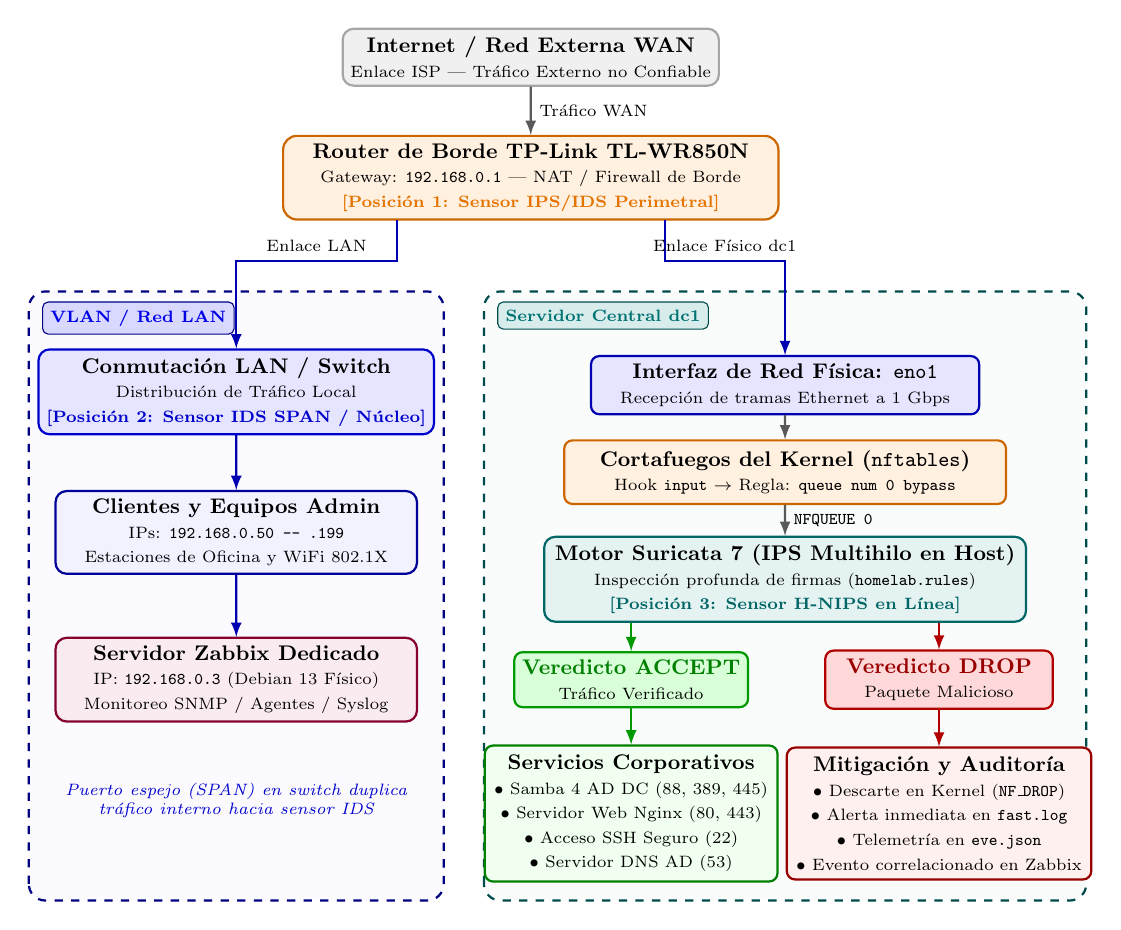
\begin{tikzpicture}[
    scale=0.85, transform shape,
    font=\linespread{0.95}\selectfont\small,
    every node/.append style={font=\linespread{0.95}\selectfont\small},
    boxwan/.style={draw=gray!70, fill=gray!12, rounded corners=4pt, minimum width=5.6cm, minimum height=0.85cm, align=center, thick},
    boxrouter/.style={draw=orange!80!black, fill=orange!12, rounded corners=5pt, minimum width=7.4cm, minimum height=1.15cm, align=center, thick},
    boxswitch/.style={draw=blue!80!black, fill=blue!10, rounded corners=4pt, minimum width=5.4cm, minimum height=1.05cm, align=center, thick},
    boxclient/.style={draw=blue!60!black, fill=blue!5, rounded corners=4pt, minimum width=5.4cm, minimum height=1.15cm, align=center, thick},
    boxzabbix/.style={draw=purple!70!black, fill=purple!8, rounded corners=4pt, minimum width=5.4cm, minimum height=1.15cm, align=center, thick},
    boxnic/.style={draw=blue!70!black, fill=blue!10, rounded corners=3pt, minimum width=5.8cm, minimum height=0.8cm, align=center, thick},
    boxnft/.style={draw=orange!80!black, fill=orange!12, rounded corners=3pt, minimum width=6.6cm, minimum height=0.95cm, align=center, thick},
    boxsuri/.style={draw=teal!80!black, fill=teal!10, rounded corners=4pt, minimum width=7.2cm, minimum height=1.2cm, align=center, thick},
    boxaccept/.style={draw=green!60!black, fill=green!15, rounded corners=3pt, minimum width=3.4cm, minimum height=0.75cm, align=center, thick},
    boxdrop/.style={draw=red!70!black, fill=red!15, rounded corners=3pt, minimum width=3.4cm, minimum height=0.75cm, align=center, thick},
    boxsvcs/.style={draw=green!50!black, fill=green!6, rounded corners=3pt, minimum width=3.6cm, align=center, thick, inner sep=4pt},
    boxlogs/.style={draw=red!60!black, fill=red!6, rounded corners=3pt, minimum width=3.6cm, align=center, thick, inner sep=4pt},
    linea/.style={-latex, thick, draw=gray!70!black},
    lineablue/.style={-latex, thick, draw=blue!70!black},
    lineagreen/.style={-latex, thick, draw=green!60!black},
    lineared/.style={-latex, thick, draw=red!70!black}
]

  % NIVEL SUPERIOR: WAN e Internet
  \node[boxwan] (wan) at (8.0, 11.6) {\textbf{Internet / Red Externa WAN}\\{\scriptsize Enlace ISP --- Tráfico Externo no Confiable}};
  \node[boxrouter] (router) at (8.0, 9.8) {\textbf{Router de Borde TP-Link TL-WR850N}\\{\scriptsize Gateway: \texttt{192.168.0.1} --- NAT / Firewall de Borde}\\{\scriptsize\textbf{\color{orange!90!black}[Posición 1: Sensor IPS/IDS Perimetral]}}};

  \draw[linea] (wan) -- node[right, font=\scriptsize]{Tráfico WAN} (router);

  % COLUMNA IZQUIERDA: Distribución LAN y Clientes (192.168.0.0/24)
  \draw[draw=blue!50!black, fill=blue!2, rounded corners=6pt, dashed, thick] (0.5, -1.0) rectangle (6.7, 8.1);
  \node[draw=blue!50!black, fill=blue!15, rounded corners=2pt, font=\scriptsize\bfseries, text=blue!90!black, anchor=north west] at (0.7, 7.95) {VLAN / Red LAN};

  \node[boxswitch] (sw) at (3.6, 6.6) {\textbf{Conmutación LAN / Switch}\\{\scriptsize Distribución de Tráfico Local}\\{\scriptsize\textbf{\color{blue!80!black}[Posición 2: Sensor IDS SPAN / Núcleo]}}};

  \node[boxclient] (clients) at (3.6, 4.5) {\textbf{Clientes y Equipos Admin}\\{\scriptsize IPs: \texttt{192.168.0.50 -- .199}}\\{\scriptsize Estaciones de Oficina y WiFi 802.1X}};

  \node[boxzabbix] (zabbix) at (3.6, 2.3) {\textbf{Servidor Zabbix Dedicado}\\{\scriptsize IP: \texttt{192.168.0.3} (Debian 13 Físico)}\\{\scriptsize Monitoreo SNMP / Agentes / Syslog}};

  \node[font=\scriptsize\itshape, text=blue!80!black, align=center] at (3.6, 0.5) {Puerto espejo (SPAN) en switch duplica\\tráfico interno hacia sensor IDS};

  % Conexión Router -> Switch LAN
  \draw[lineablue] ([xshift=-2.0cm]router.south) -- ++(0,-0.6) -| node[above, pos=0.25, font=\scriptsize]{Enlace LAN} (sw.north);
  \draw[lineablue] (sw) -- (clients);
  \draw[lineablue] (clients) -- (zabbix);

  % COLUMNA DERECHA: Servidor Central dc1 (IPS en Host)
  \draw[draw=teal!60!black, fill=teal!2, rounded corners=6pt, dashed, thick] (7.3, -1.0) rectangle (16.3, 8.1);
  \node[draw=teal!60!black, fill=teal!15, rounded corners=2pt, font=\scriptsize\bfseries, text=teal!90!black, anchor=north west] at (7.5, 7.95) {Servidor Central dc1};

  \node[boxnic] (nic) at (11.8, 6.7) {\textbf{Interfaz de Red Física: \texttt{eno1}}\\{\scriptsize Recepción de tramas Ethernet a 1 Gbps}};

  \node[boxnft] (nft) at (11.8, 5.4) {\textbf{Cortafuegos del Kernel (\texttt{nftables})}\\{\scriptsize Hook \texttt{input} $\rightarrow$ Regla: \texttt{queue num 0 bypass}}};

  \node[boxsuri] (suri) at (11.8, 3.8) {\textbf{Motor Suricata 7 (IPS Multihilo en Host)}\\{\scriptsize Inspección profunda de firmas (\texttt{homelab.rules})}\\{\scriptsize\textbf{\color{teal!80!black}[Posición 3: Sensor H-NIPS en Línea]}}};

  % Ramificación Veredictos
  \node[boxaccept] (accept) at (9.5, 2.3) {\textbf{\color{green!50!black}Veredicto ACCEPT}\\{\scriptsize Tráfico Verificado}};
  \node[boxdrop] (drop) at (14.1, 2.3) {\textbf{\color{red!60!black}Veredicto DROP}\\{\scriptsize Paquete Malicioso}};

  \node[boxsvcs] (svcs) at (9.5, 0.3) {\textbf{Servicios Corporativos}\\{\scriptsize $\bullet$ Samba 4 AD DC (88, 389, 445)}\\{\scriptsize $\bullet$ Servidor Web Nginx (80, 443)}\\{\scriptsize $\bullet$ Acceso SSH Seguro (22)}\\{\scriptsize $\bullet$ Servidor DNS AD (53)}};

  \node[boxlogs] (logs) at (14.1, 0.3) {\textbf{Mitigación y Auditoría}\\{\scriptsize $\bullet$ Descarte en Kernel (\texttt{NF\_DROP})}\\{\scriptsize $\bullet$ Alerta inmediata en \texttt{fast.log}}\\{\scriptsize $\bullet$ Telemetría en \texttt{eve.json}}\\{\scriptsize $\bullet$ Evento correlacionado en Zabbix}};

  % Conexión Router -> dc1
  \draw[lineablue] ([xshift=2.0cm]router.south) -- ++(0,-0.6) -| node[above, pos=0.25, font=\scriptsize]{Enlace Físico dc1} (nic.north);

  % Conexiones dentro de dc1
  \draw[linea] (nic) -- (nft);
  \draw[linea] (nft) -- node[right, font=\scriptsize\ttfamily]{NFQUEUE 0} (suri);

  \draw[lineagreen] (suri.south -| accept.north) -- (accept.north);
  \draw[lineagreen] (accept.south) -- (svcs.north);

  \draw[lineared] (suri.south -| drop.north) -- (drop.north);
  \draw[lineared] (drop.south) -- (logs.north);

\end{tikzpicture}%
}{Elaboración propia.}
\end{minipage}
\end{center}

\subsubsection{Mecanismo de Protección Integral del Servidor dc1}

Para comprender con exactitud de qué manera las herramientas seleccionadas blindan al servidor centralizado de la organización, es necesario examinar el flujo de defensa a nivel de bajo nivel en el kernel y su correspondencia puerto a puerto con los servicios corporativos alojados en \texttt{dc1}.

\paragraph{Flujo de Intercepción y Decisión en Núcleo (Kernel-level Pipeline).}
El servidor \texttt{dc1} (\texttt{192.168.0.2}) implementa una defensa activa que opera a nivel de paquete antes de que los datos alcancen la memoria de las aplicaciones:

\begin{enumerate}
  \item \textbf{Ingreso por Interfaz Física (\texttt{eno1}):} Las tramas Ethernet provenientes de los clientes o del enrutador son recibidas por el controlador de red del kernel Linux.
  \item \textbf{Evaluación en la Cadena \texttt{input} de \texttt{nftables}:} Antes de que el paquete sea entregado a la pila de transporte TCP/UDP local, el hook \texttt{input} del cortafuegos evalúa la regla de redirección:
\begin{lstlisting}[language=bash]
meta l4proto tcp ct state new,established counter queue num 0 bypass
\end{lstlisting}
  \item \textbf{Transferencia a Espacio de Usuario vía \texttt{NFQUEUE}:} El paquete es copiado hacia la cola número 0 administrada por el subsistema Netfilter en memoria compartida del kernel.
  \item \textbf{Inspección Profunda Multihilo en Suricata 7:} Un hilo de Suricata extrae el paquete de la cola, ejecuta el reensamblaje del flujo TCP, normaliza el protocolo de capa de aplicación y evalúa concurrentemente las firmas locales (\texttt{homelab.rules}) aceleradas por Intel Hyperscan.
  \item \textbf{Emisión del Veredicto en Microsegundos:}
    \begin{itemize}
      \item \textbf{Veredicto ACCEPT (Tráfico Legítimo):} Suricata emite la instrucción \texttt{NF\_ACCEPT} al kernel. El paquete continúa su flujo normal y es entregado al zócalo (*socket*) del servicio de destino (Samba AD, Nginx, BIND9, SSH).
      \item \textbf{Veredicto DROP (Tráfico Malicioso):} Si el payload coincide con una firma de descarte, Suricata emite \texttt{NF\_DROP}. El kernel destruye el búfer de memoria del paquete de inmediato. La aplicación destinataria jamás recibe la petición, el atacante sufre una desconexión abrupta (*timeout* o *reset*) y la vulnerabilidad potencial queda completamente inaccesible.
    \end{itemize}
  \item \textbf{Garantía de Continuidad Operativa (*Fail-Open*):} Gracias al parámetro \texttt{bypass}, si el motor de Suricata se sobrecarga, se detiene o se reinicia, el kernel permite el paso directo del tráfico para evitar una caída no planificada de la red corporativa.
\end{enumerate}

\paragraph{Matriz de Protección por Servicio y Puerto Corporativo.}
La Tabla~\ref{tab:matriz-proteccion-dc1} detalla la correspondencia entre los servicios residentes en \texttt{dc1}, los puertos expuestos, las amenazas mitigadas y el mecanismo técnico que ejerce Suricata.

\begin{table}[H]
\centering
\caption{Matriz de Protección Defensiva por Servicio y Puerto en dc1}
\label{tab:matriz-proteccion-dc1}
\contenidoConFuente{%
  \begin{tablaAPA}
  \begin{tabular}{L{3.0cm}L{2.0cm}L{4.8cm}L{4.6cm}}
  \toprule
  \textbf{Servicio en dc1} & \textbf{Puertos} & \textbf{Amenazas Mitigadas} & \textbf{Mecanismo de Suricata} \\
  \midrule
  \textbf{Active Directory DC (Kerberos)} & 88 (TCP/UDP) & Fuerza bruta contra contraseñas, enumeración de usuarios, ataques AS-REP Roasting. & Regla de umbral (\texttt{threshold}) con firma \texttt{sid:9000030} y descarte preventivo. \\
  \textbf{Active Directory DC (LDAP/LDAPS)} & 389, 636 (TCP) & Reconocimiento masivo de objetos del dominio, inyecciones de filtros LDAP, volcado de atributos. & Decodificador nativo de capa 7 para transacciones LDAP y alertas estructuradas. \\
  \textbf{Samba File Server (SMB/CIFS)} & 445 (TCP) & Explotación de vulnerabilidades remotas (tipo EternalBlue MS17-010), ransomware en recursos compartidos. & Decodificador nativo SMB2/SMB3, inspección de comandos y extracción de hashes de archivos. \\
  \textbf{Servidor Web Nginx} & 80, 443 (TCP) & Inyecciones SQL (SQLi), ejecución remota de comandos (RCE, Log4Shell), traversales de directorio. & Regla IPS con acción \texttt{drop} en línea (\texttt{sid:9000002}) que bloquea el payload antes del daemon web. \\
  \textbf{Servicio de Nombres (DNS AD)} & 53 (UDP/TCP) & Consultas malformadas, envenenamiento de caché DNS, exfiltración por túneles encubiertos DNS. & Parser nativo de protocolo DNS con validación de anomalías de RFC en tiempo real. \\
  \textbf{Acceso Remoto Seguro (SSH)} & 22 (TCP) & Escaneo sigiloso de puertos, ataques automatizados de diccionario y fuerza bruta SSH. & Correlación de banderas TCP y rate-limiting en conjunto con la telemetría de \texttt{eve.json}. \\
  \textbf{Capa de Red Global} & Todos & Cartografiado sigiloso mediante escaneos TCP NULL y TCP XMAS. & Detección de combinaciones ilícitas de banderas TCP (\texttt{flags:0} y \texttt{flags:FPU}). \\
  \bottomrule
  \end{tabular}
  \end{tablaAPA}%
}{Elaboración propia.}
\end{table}

% ----------------------------------------------------------------------------
\subsection{Implementación y Validación Práctica en el Laboratorio}

La solución analizada fue desplegada en el servidor \texttt{dc1} mediante un módulo técnico integrado, disponible en el repositorio bajo la ruta \texttt{server/suricata/}. A continuación se describen las reglas implementadas y las pruebas empíricas efectuadas.

\subsubsection{Despliegue de Reglas de Seguridad Locales}

Se estructuró el archivo de firmas de seguridad local \texttt{homelab.rules}, enfocado en la mitigación de los vectores de ataque más habituales en la organización:

\begin{itemize}
  \item \textbf{Firma de Bloqueo IPS (Prueba en Línea):}
\begin{lstlisting}[language=bash]
drop tcp any any -> $HOME_NET $HTTP_PORTS (msg:"[HOMELAB-IPS-DROP] Bloqueo HTTP: Carga maliciosa en aplicacion web"; flow:to_server,established; content:"MALICIOUS_SIMULATION_ATTACK"; nocase; sid:9000002; rev:1;)
\end{lstlisting}
  \item \textbf{Firma de Alerta IDS (Sonda Pasiva):}
\begin{lstlisting}[language=bash]
alert tcp any any -> $HOME_NET any (msg:"[HOMELAB-IDS-ALERT] Sonda de prueba detectada (TEST_PROBE_ALERT_ONLY)"; flow:to_server,established; content:"TEST_PROBE_ALERT_ONLY"; nocase; sid:9000010; rev:1;)
\end{lstlisting}
  \item \textbf{Protección contra Escaneos Sigilosos:} Detección de paquetes con banderas TCP vacías (escaneos NULL) o banderas combinadas FPU (escaneos XMAS):
\begin{lstlisting}[language=bash]
alert tcp any any -> $HOME_NET any (msg:"[HOMELAB-IDS-ALERT] Reconocimiento de red: Escaneo TCP NULL detectado"; flags:0; sid:9000020; rev:1;)
alert tcp any any -> $HOME_NET any (msg:"[HOMELAB-IDS-ALERT] Reconocimiento de red: Escaneo TCP XMAS detectado"; flags:FPU; sid:9000021; rev:1;)
\end{lstlisting}
  \item \textbf{Protección de Kerberos y Active Directory:} Detección de sondeos masivos orientados a saturar o enumerar usuarios en el puerto 88:
\begin{lstlisting}[language=bash]
alert tcp any any -> $HOME_NET 88 (msg:"[HOMELAB-IDS-ALERT] Sondeo continuo o sospechoso al servicio Kerberos del AD DC"; flags:S; threshold:type both, track by_src, count 15, seconds 5; sid:9000030; rev:1;)
\end{lstlisting}
\end{itemize}

\subsubsection{Guía Operativa y Comandos de Administración de Suricata}

Para la correcta administración, supervisión y puesta en marcha de Suricata en un entorno de producción sobre GNU/Linux Debian, se estructuró un conjunto estandarizado de comandos y utilitarios operativos en el servidor \texttt{dc1}:

\paragraph{1. Gestión del Demonio del Sistema mediante Systemd.}
Al haber sido instalado de forma nativa en el sistema operativo host, el ciclo de vida del motor de seguridad se controla mediante el gestor del sistema \texttt{systemd}:
\begin{lstlisting}[language=bash]
# Consultar el estado operativo y metricas de hilos de Suricata:
sudo systemctl status suricata

# Iniciar, detener o reiniciar el motor de deteccion:
sudo systemctl start suricata
sudo systemctl stop suricata
sudo systemctl restart suricata

# Recargar firmas en caliente sin interrumpir la captura de trafico:
sudo systemctl reload suricata
\end{lstlisting}

\paragraph{2. Validación Preventiva de Configuración y Sintaxis (-T).}
Antes de aplicar cambios a las firmas de seguridad o a los parámetros de red en \texttt{suricata.yaml}, es una buena práctica de ingeniería ejecutar el modo de prueba (\textit{Test Mode}):
\begin{lstlisting}[language=bash]
# Validar la sintaxis de configuracion y el parseo de todas las reglas:
sudo suricata -T -c /etc/suricata/suricata.yaml -v
\end{lstlisting}
El parámetro \texttt{-T} inicializa los motores de decodificación y compila las firmas con Hyperscan en memoria. Si no se detectan inconsistencias, finaliza con código de salida 0 (\textit{Configuration provided was successfully tested}).

\paragraph{3. Alternancia Dinámica de Modos Operativos (IDS vs IPS).}
Para gestionar la transición entre el modo pasivo (sólo alertas) y el modo preventivo (descarte en línea), se dispone del utilitario interactivo \texttt{server/suricata/ips-toggle.sh}:
\begin{lstlisting}[language=bash]
# Activar modo IPS (inserta regla NFQUEUE 0 bypass en la cadena input de nftables):
sudo bash server/suricata/ips-toggle.sh --ips

# Retornar a modo IDS pasivo (remueve la regla de desvio en nftables):
sudo bash server/suricata/ips-toggle.sh --ids

# Comprobar el modo operativo activo y las alertas mas recientes:
bash server/suricata/ips-toggle.sh --status
\end{lstlisting}

Asimismo, la verificación directa de la cola en el subsistema del kernel se realiza mediante:
\begin{lstlisting}[language=bash]
# Inspeccionar las reglas de cola activas en el cortafuegos del kernel:
sudo nft list table inet filter | grep queue
\end{lstlisting}

\paragraph{4. Supervisión y Auditoría de Bitácoras en Tiempo Real.}
Suricata genera registros complementarios en el directorio \texttt{/var/log/suricata/}:
\begin{lstlisting}[language=bash]
# Monitoreo en vivo de alertas tradicionales y bloqueos (fast.log):
sudo tail -f /var/log/suricata/fast.log

# Monitoreo estructurado de eventos JSON filtrando alertas y descartes (eve.json):
sudo tail -f /var/log/suricata/eve.json | jq 'select(.event_type=="alert" or .event_type=="drop")'

# Estadisticas operativas de rendimiento y contadores de paquetes:
sudo tail -n 30 /var/log/suricata/stats.log
\end{lstlisting}

\paragraph{5. Actualización Continua de Firmas de Seguridad.}
La sincronización periódica de firmas de amenazas comunitarias se ejecuta mediante:
\begin{lstlisting}[language=bash]
# Descargar el ultimo conjunto de firmas de Emerging Threats Open:
sudo suricata-update

# Recargar el motor para aplicar las nuevas reglas descargadas:
sudo suricatasc -c reload-rules
\end{lstlisting}

\paragraph{6. Ejecución de la Batería de Pruebas de Validación.}
Para verificar el funcionamiento integral de la solución en laboratorio, se ejecuta la suite automatizada:
\begin{lstlisting}[language=bash]
# Ejecutar pruebas E2E de envio de sondas y payloads maliciosos:
sudo bash server/suricata/test-ids-ips.sh
\end{lstlisting}

\subsubsection{Pruebas Experimentales de Laboratorio}

La suite de validación automatizada (\texttt{server/suricata/test-ids-ips.sh}) permitió demostrar experimentalmente la dualidad funcional entre el modo IDS y el modo IPS:

\paragraph{Caso 1: Demostración en Modo IDS (Detección Pasiva).}
Con el sensor operando sobre zócalos \texttt{AF\_PACKET}, se transmitió una solicitud HTTP dirigida al servidor con la cadena \texttt{TEST\_PROBE\_ALERT\_ONLY}.
\begin{itemize}
  \item \textbf{Comportamiento de Red:} La conexión TCP completó exitosamente el saludo de tres vías (*three-way handshake*) y el servidor web entregó el código de estado HTTP 200 al cliente.
  \item \textbf{Registro Generado en \texttt{fast.log}:}
\begin{lstlisting}[style=terminal]
10/24/2026-11:45:10.102341 [**] [1:9000010:1] [HOMELAB-IDS-ALERT] Sonda de prueba detectada (TEST_PROBE_ALERT_ONLY) [**] [Classification: Misc activity] [Priority: 3] {TCP} 192.168.0.50:48210 -> 192.168.0.2:80
\end{lstlisting}
  \item \textbf{Conclusión:} El IDS cumplió su rol de observador no invasivo, alertando sobre la presencia de la firma sin afectar el tráfico.
\end{itemize}

\paragraph{Caso 2: Demostración en Modo IPS (Prevención y Descarte Activo).}
Se activó el modo IPS mediante el script \texttt{ips-toggle.sh --ips}, inyectando la regla \texttt{queue num 0 bypass} en la cadena \texttt{input} de \texttt{nftables}. Posteriormente, se envió una solicitud HTTP simulando un vector de exploit con el payload \texttt{MALICIOUS\_SIMULATION\_ATTACK}.
\begin{itemize}
  \item \textbf{Comportamiento de Red:} La conexión del cliente se abortó de manera inmediata con un error de tiempo de espera agotado (*timeout*) o terminación forzada (*connection reset*). El paquete jamás fue recibido por el proceso de Nginx ni por la aplicación interna.
  \item \textbf{Registro Generado en \texttt{fast.log}:}
\begin{lstlisting}[style=terminal]
10/24/2026-11:48:22.589124 [Drop] [**] [1:9000002:1] [HOMELAB-IPS-DROP] Bloqueo HTTP: Carga maliciosa en aplicacion web (MALICIOUS_SIMULATION_ATTACK) [**] [Classification: Web Application Attack] [Priority: 1] {TCP} 192.168.0.50:51402 -> 192.168.0.2:80
\end{lstlisting}
  \item \textbf{Conclusión:} La etiqueta \texttt{[Drop]} confirma que Suricata emitió el veredicto de descarte al módulo NFQUEUE del kernel Linux, neutralizando proactivamente la amenaza en tiempo real.
\end{itemize}

\paragraph{Caso 3: Telemetría Estructurada en \texttt{eve.json}.}
Adicionalmente, se confirmó que cada evento de bloqueo genera un registro enriquecido en formato JSON que detalla el flujo, direcciones físicas MAC, payload transmitido y códigos de clasificación:

\begin{lstlisting}[style=terminal]
{
  "timestamp": "2026-10-24T11:48:22.589124-0400",
  "flow_id": 819203918239,
  "event_type": "drop",
  "src_ip": "192.168.0.50",
  "src_port": 51402,
  "dest_ip": "192.168.0.2",
  "dest_port": 80,
  "proto": "TCP",
  "action": "blocked",
  "alert": {
    "action": "drop",
    "signature_id": 9000002,
    "signature": "[HOMELAB-IPS-DROP] Bloqueo HTTP: Carga maliciosa en aplicacion web"
  }
}
\end{lstlisting}
